\begin{enumerate}
    \item On obtient la figure sivante :
    
    \medskip
    \begin{tikzpicture}[x=1cm,y=1cm]                
    \draw (0,0) -- (1,0); 
    \draw (2,0) -- (2,-1);
    \draw (2,-2) -- (1,-2); 
    \draw (0,-2) -- (0,-1);
\end{tikzpicture}
    \item Elle doit modifier le « répéter 4 fois » et supprimer « tourner … »
    
    \begin{scratch}[scale=.7,print]
        \blockinit{quand \greenflag est cliqué}
        \blockpen{effacer tout}
        \blockmove{aller à x: \ovalnum0 y: \ovalnum0}
        \blockmove{s’orienter à \ovalnum{90} degrés}    
        \blockrepeat{répéter \ovalnum{8} fois}
        {
        \blockpen{stylo en position d’écriture}
        \blockmove{avancer de \ovalnum{10}}
        \blockpen{relever le stylo}
        \blockmove{avancer de \ovalnum{10}}            
        }
    \end{scratch}

    \item 
    \begin{enumerate}
        \item Il doit modifier le « répéter 4 fois » et modifier l’angle dans « tourner … »

        \begin{scratch}[scale=.7,print]
            \blockinit{quand \greenflag est cliqué}
            \blockpen{effacer tout}
            \blockmove{aller à x: \ovalnum0 y: \ovalnum0}
            \blockmove{s’orienter à \ovalnum{90} degrés}    
            \blockrepeat{répéter \ovalnum{8} fois}
            {
            \blockpen{stylo en position d’écriture}
            \blockmove{avancer de \ovalnum{10}}
            \blockpen{relever le stylo}
            \blockmove{avancer de \ovalnum{10}}   
            \blockmove{tourner \turnright{} de \ovalnum{45} degrés}         
            }
        \end{scratch}

        \item Pour passer d’un tiret à l’autre on a une rotation de centre $O$ d’angle $45$ \degree dans le sens des aiguilles d’une montre.
        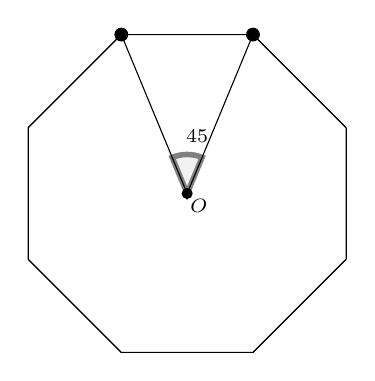
\begin{tikzpicture}[x=.55cm,y=.55cm]            
            \draw (-8.749207731733707,-1.9847765108368634) -- (-5.7092077317337075,-1.9847765108368634) -- (-3.559603116926604,0.16482810397024017) -- (-3.5596031169266036,3.2048281039702387) -- (-5.7092077317337075,5.354432718777343) -- (-8.749207731733707,5.3544327187773435) -- (-10.89881234654081,3.20482810397024) -- (-10.898812346540812,0.16482810397024128) -- cycle;
            \draw [shift={(-7.229207731733707,1.6848281039702409)},line width=2pt,color=gray,fill=gray,fill opacity=0.1] (0,0) -- (67.5:0.9017264497000701) arc (67.5:112.5:0.9017264497000701) -- cycle;
            \draw (-8.749207731733707,-1.9847765108368634)-- (-5.7092077317337075,-1.9847765108368634);
            \draw (-5.7092077317337075,-1.9847765108368634)-- (-3.559603116926604,0.16482810397024017);
            \draw (-3.559603116926604,0.16482810397024017)-- (-3.5596031169266036,3.2048281039702387);
            \draw (-3.5596031169266036,3.2048281039702387)-- (-5.7092077317337075,5.354432718777343);
            \draw (-5.7092077317337075,5.354432718777343)-- (-8.749207731733707,5.3544327187773435);
            \draw (-8.749207731733707,5.3544327187773435)-- (-10.89881234654081,3.20482810397024);
            \draw (-10.89881234654081,3.20482810397024)-- (-10.898812346540812,0.16482810397024128);
            \draw (-10.898812346540812,0.16482810397024128)-- (-8.749207731733707,-1.9847765108368634);
            \draw (-7.229207731733707,1.6848281039702409)-- (-8.749207731733707,5.3544327187773435);
            \draw (-7.229207731733707,1.6848281039702409)-- (-5.7092077317337075,5.354432718777343);
            \begin{scriptsize}
            \fill (-5.7092077317337075,5.354432718777343) circle (2.5pt);
            \fill (-8.749207731733707,5.3544327187773435) circle (2.5pt);
            \fill (-7.229207731733707,1.6848281039702409) circle (2pt);
            \draw (-6.960197258332642,1.4033186920234155) node {$O$};
            \draw (-7,3) node {$45\textrm{\degre}$};
            \end{scriptsize}
            \end{tikzpicture}
    \end{enumerate}
\end{enumerate}